\imagefigure{%
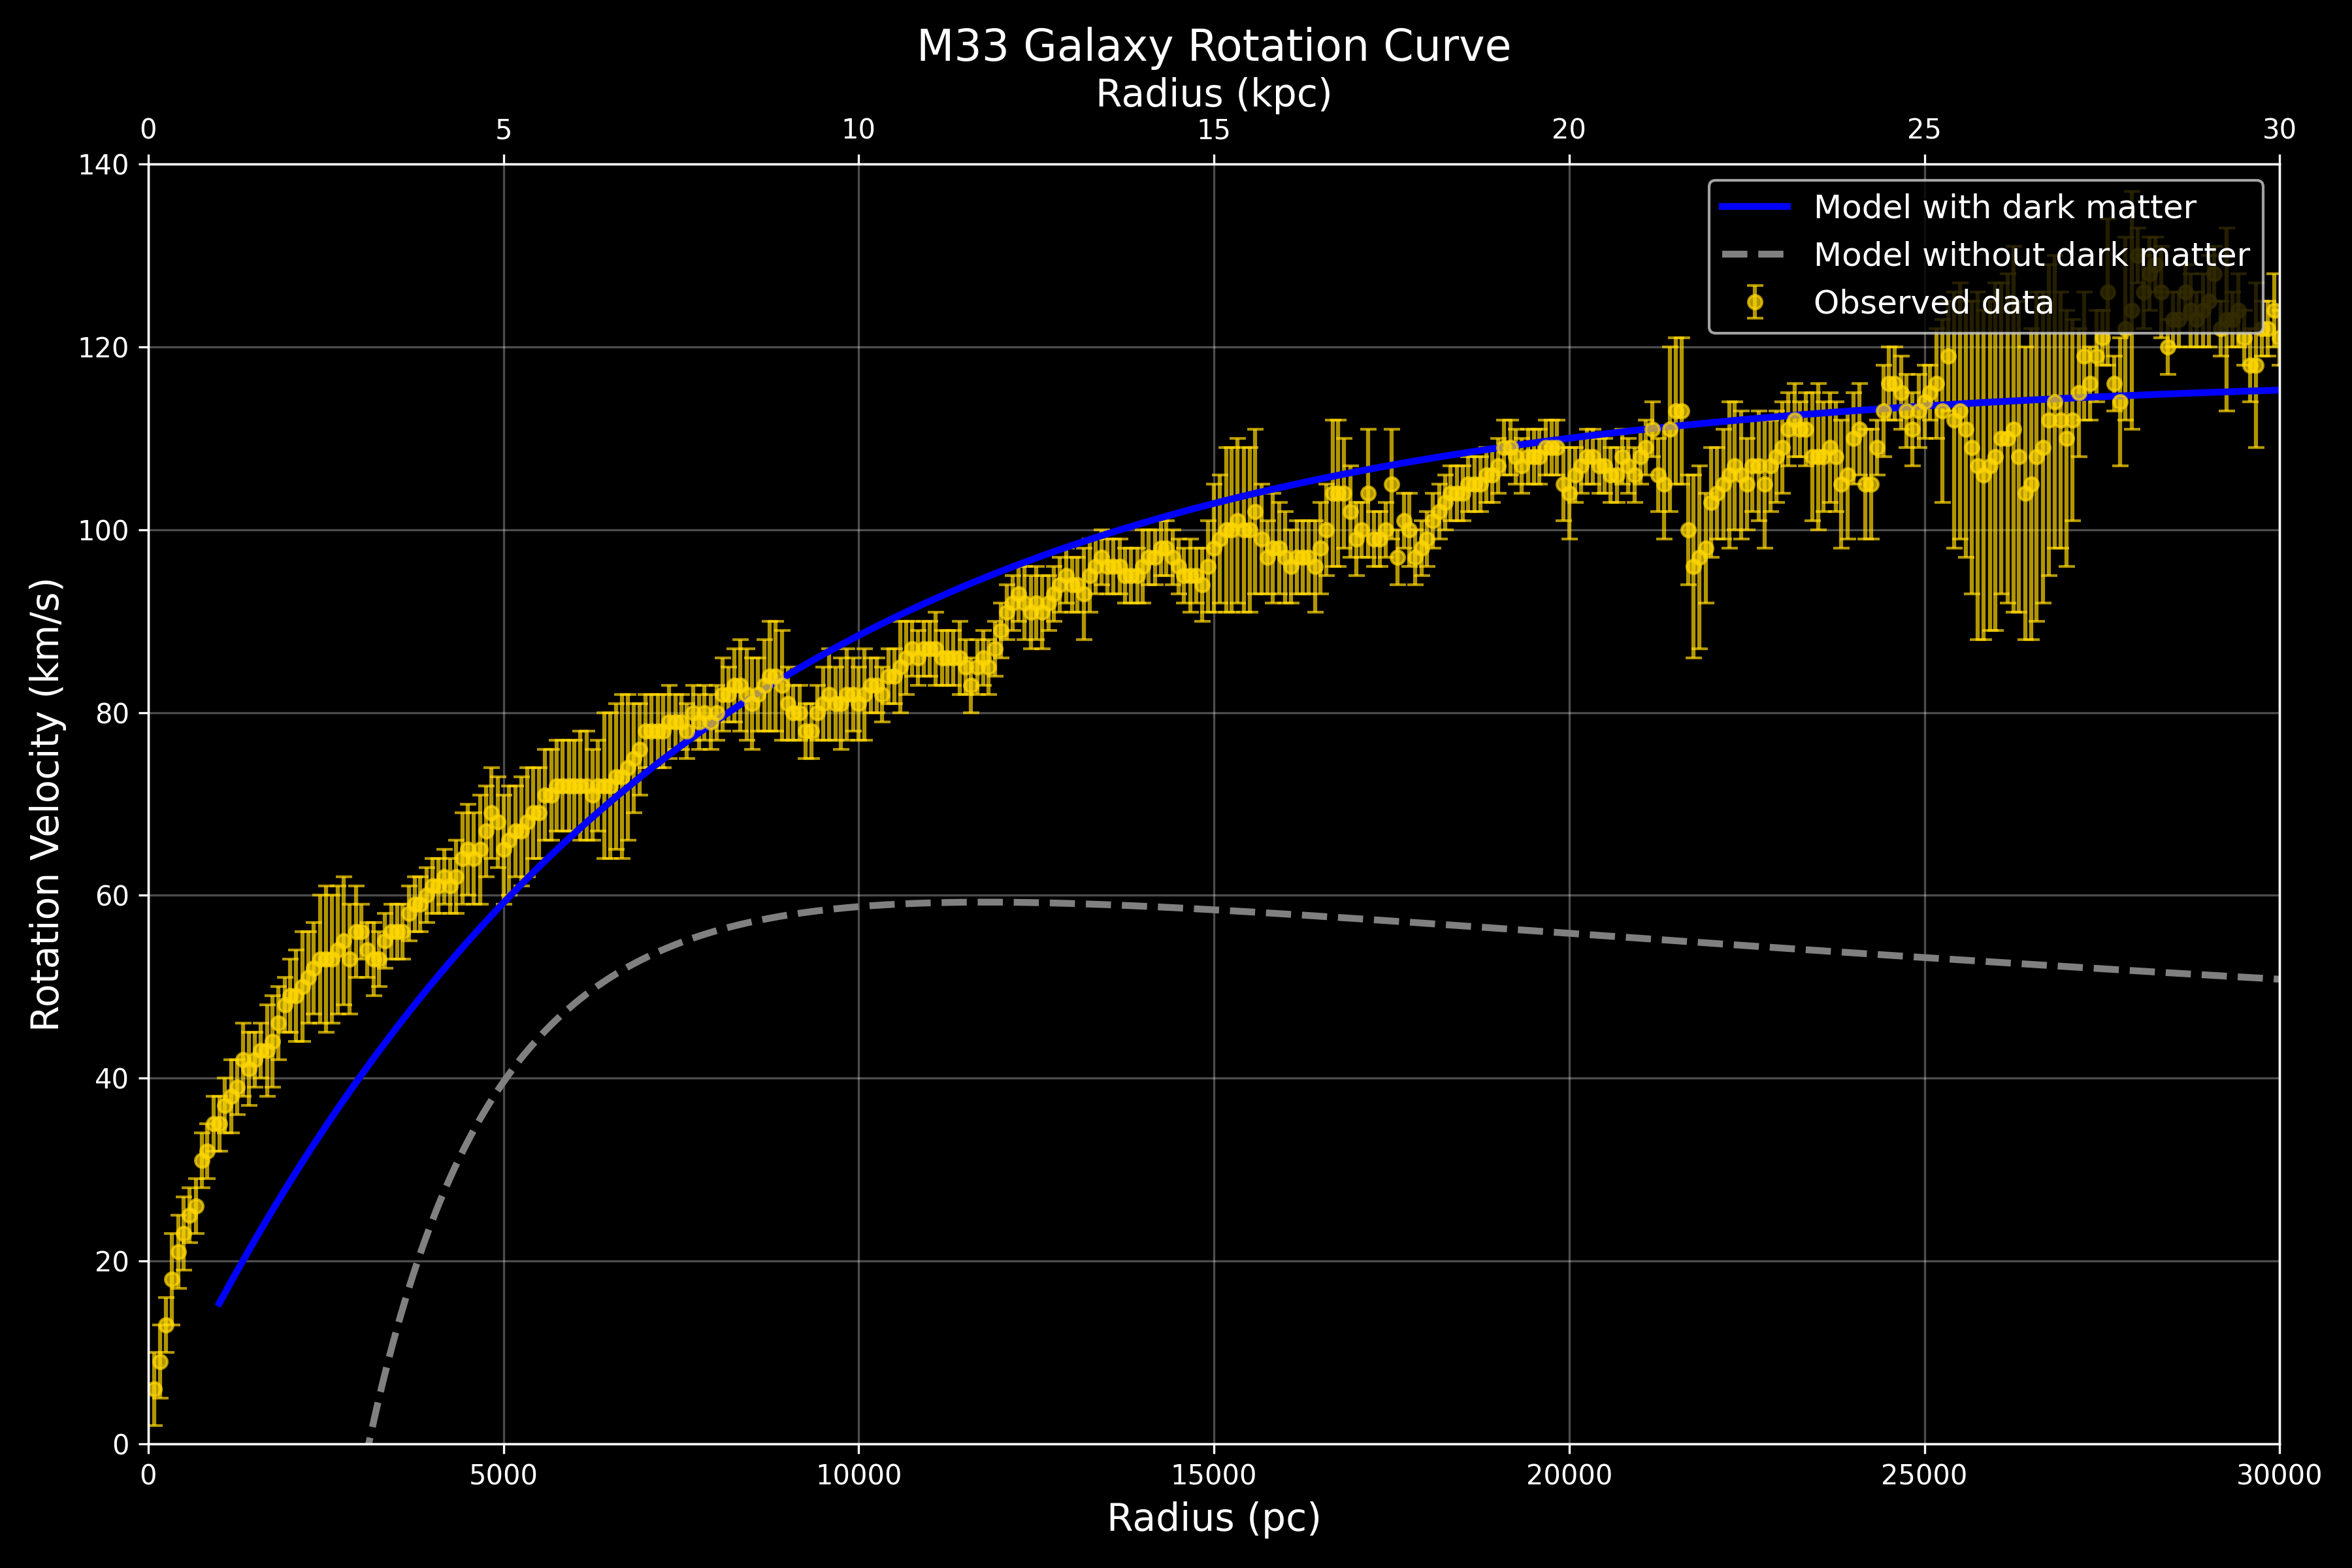
\includegraphics[width=0.75\textwidth]{37_DarkMatterEvidence/m33_rotation_curve.png}
}{%
\textbf{M33 Galaxy Rotation Curve.} The rotation curve of the M33 galaxy (Triangulum Galaxy) demonstrates the need for dark matter in galaxies. Yellow points represent observed H$\alpha$ spectroscopic data collected at the Observatoire du Mont Megantic, showing rotation velocities with error bars at different galactocentric radii. The solid blue line shows a model that includes dark matter contribution, following the function $v = M \cdot (1 - e^{-r/R})$, which maintains high velocities at large radii. The gray dashed line represents a toy model based only on visible baryonic matter which cannot account for the observed rotation velocities in the outer regions of the galaxy. This discrepancy provides compelling evidence for the presence of a dark matter halo extending far beyond the visible disk of M33.

\vspace{0.5em}
\small{Figure generated by me using data points from Kam et al. (2015), "The H$\alpha$ rotation curve of M33" (MNRAS, 449, 4048). The fitted curved are not from the literature and for illustrative purposes only.}
}